\chapter{Contexto y estado del arte}\label{chap:objetivos}

El presente capítulo tiene como objetivo contextualizar el trabajo dentro del ámbito tecnológico actual, abordando los conceptos fundamentales, tecnologías relevantes y principales herramientas empleadas en sistemas distribuidos y arquitecturas de microservicios. Se describen los antecedentes teóricos y técnicos relacionados con la observabilidad, así como los enfoques más destacados en la industria y la academia.

Además, se analizan trabajos relacionados y se justifica la elección de las tecnologías utilizadas en esta propuesta. Finalmente, se extraen conclusiones que fundamentan la pertinencia y el valor añadido del enfoque desarrollado en este Trabajo Fin de Máster.

\section{Contextualización y antecedentes}\label{sec:contextyantec}

La creciente complejidad de los sistemas distribuidos, en particular los basados en arquitecturas de microservicios, ha impulsado el desarrollo y adopción de nuevas prácticas y herramientas para la gestión eficiente de estos entornos. En este contexto, la observabilidad se ha convertido en un elemento clave para garantizar la fiabilidad, el mantenimiento y la evolución del software \cite{Ramaswamy2024, Bhosale2022, Zhang2020}.

Una arquitectura de microservicios consiste en la descomposición de una aplicación en múltiples servicios pequeños, autónomos y desplegables de forma independiente \cite{Newman2015, Dragoni2017, Dragoni2017Preprint}. Esta forma de organización permite una mayor escalabilidad y flexibilidad. No obstante, introduce importantes desafíos en cuanto al monitoreo, la gestión de logs y la trazabilidad de peticiones. A diferencia de los sistemas monolíticos, donde el diagnóstico de errores puede realizarse de forma centralizada, los microservicios requieren soluciones que permitan observar el comportamiento distribuido del sistema \cite{Singh2021}.

El paradigma DevOps ha transformado también el ciclo de vida del software, promoviendo la automatización del desarrollo, despliegue y operación de aplicaciones. Sin embargo, para que este enfoque funcione eficazmente, es necesario contar con sistemas que permitan observar el estado de los servicios en todo momento. La observabilidad se basa en tres pilares fundamentales: monitoreo, logging y tracing \cite{Google2020, CNCF2023, Ramaswamy2024}. Los tres pilares son complementarios: las métricas permiten medir rendimiento y disponibilidad, los logs registran eventos de manera detallada y las trazas facilitan seguir el recorrido de una solicitud a través de múltiples servicios.

Las principales tecnologías que abordan estos aspectos incluyen:

\begin{itemize}
	\item \textbf{Prometheus y Grafana}, para recolección y visualización de métricas en tiempo real.
	\item \textbf{ELK Stack} (Elasticsearch, Logstash y Kibana), para gestión y análisis de logs.
	\item \textbf{Jaeger y OpenTelemetry}, para trazabilidad distribuida en entornos con múltiples servicios.
\end{itemize}

Estas herramientas cuentan con soporte comunitario activo y son utilizadas por empresas que operan sistemas complejos a gran escala, como Netflix, Uber y SoundCloud. Su adopción ha permitido identificar patrones de fallo, cuellos de botella y realizar diagnósticos proactivos en producción \cite{UberCase2018, NetflixCase2019, Villamizar2021}.

Asimismo, tecnologías como \textbf{Docker} y \textbf{Kubernetes} se han convertido en el estándar para el despliegue y orquestación de microservicios. A través de ellas, es posible simular entornos de producción en local —por ejemplo, mediante Minikube— y automatizar despliegues con herramientas como Helm y Ansible, facilitando tanto la reproducibilidad como la escalabilidad del sistema \cite{Lee2023, CNCFSecurity2022}. Esto garantiza que los microservicios puedan ser desplegados, escalados y observados de manera coherente en entornos dinámicos.

Para el desarrollo de los microservicios, se utilizará \textbf{Spring Boot}, un framework ampliamente adoptado que permite crear aplicaciones independientes y listas para producción. Spring Boot ofrece integración nativa con métricas, logging y trazabilidad, lo que facilita la instrumentación de servicios y su integración con herramientas de observabilidad como Prometheus, Grafana y Jaeger \cite{Newman2015, Smith2022}.

En resumen, el contexto actual exige soluciones de observabilidad integradas, configurables, automatizadas y adaptadas a entornos altamente dinámicos, donde la fiabilidad del sistema depende de la capacidad de observar y reaccionar rápidamente ante eventos adversos.

% -----------------------------
% Figura 1: Flujos de servicios
% -----------------------------
\begin{figure}[H]
	\centering
	\caption{Diagrama de microservicios y flujos de llamadas.}
	\shorthandoff{>}
	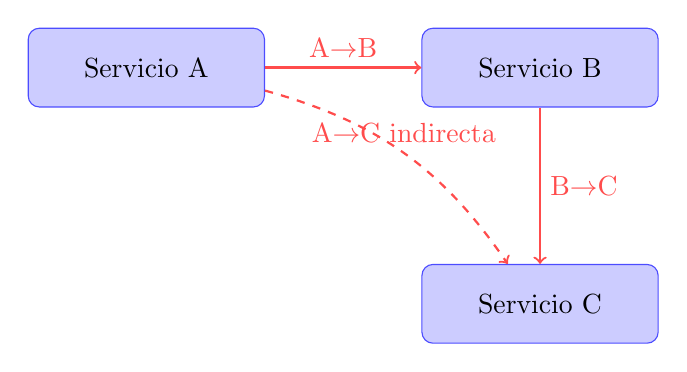
\begin{tikzpicture}[
		service/.style={rectangle, draw=blue!70, fill=blue!20, rounded corners, minimum width=3cm, minimum height=1cm, align=center},
		call/.style={->, thick, red!70},
		indirect/.style={->, thick, red!70, dashed}
		]
		
		\node[service] (A) at (0,0) {Servicio A};
		\node[service] (B) at (5,0) {Servicio B};
		\node[service] (C) at (5,-3) {Servicio C};
		
		\draw[call] (A) -- (B) node[midway, above] {A$\to$B};
		\draw[call] (B) -- (C) node[midway, right] {B$\to$C};
		\draw[indirect, bend left=20] (A) to node[midway, above] {A$\to$C indirecta} (C);
		
	\end{tikzpicture}
	\caption*{\footnotesize Fuente: Elaboración propia.}
	\label{fig:microservicios-flujos}
\end{figure}

% -----------------------------
% Figura 2: Servicios y observabilidad
% -----------------------------
\begin{figure}[H]
	\centering
	\caption{Servicios y pilares de observabilidad}
	\shorthandoff{>}
	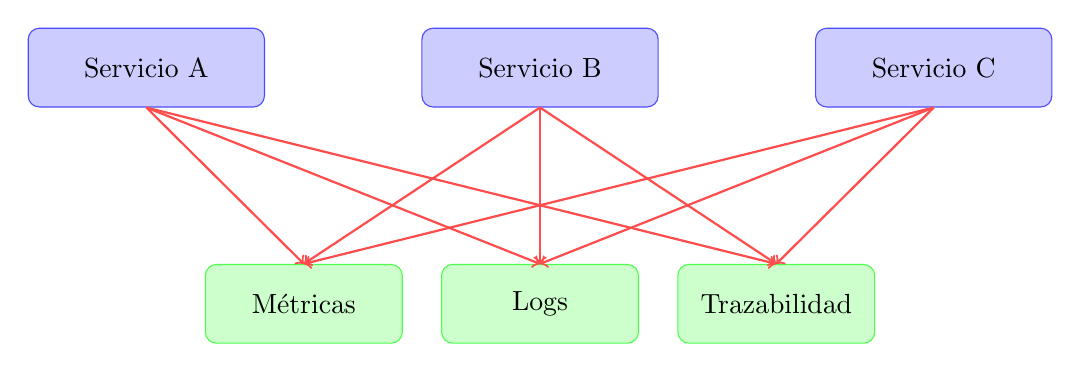
\begin{tikzpicture}[
		service/.style={rectangle, draw=blue!70, fill=blue!20, rounded corners, minimum width=3cm, minimum height=1cm, align=center},
		pillar/.style={rectangle, draw=green!70, fill=green!20, rounded corners, minimum width=2.5cm, minimum height=1cm, align=center},
		call/.style={->, thick, red!70}
		]
		
		\node[service] (A) at (0,0) {Servicio A};
		\node[service] (B) at (5,0) {Servicio B};
		\node[service] (C) at (10,0) {Servicio C};
		
		\node[pillar] (metrics) at (2,-3) {Métricas};
		\node[pillar] (logs) at (5,-3) {Logs};
		\node[pillar] (tracing) at (8,-3) {Trazabilidad};
		
		\foreach \s in {A,B,C} {
			\draw[call] (\s.south) -- (metrics.north);
			\draw[call] (\s.south) -- (logs.north);
			\draw[call] (\s.south) -- (tracing.north);
		}
		
	\end{tikzpicture}
	\caption*{\footnotesize Fuente: Elaboración propia.}
	\label{fig:microservicios-observabilidad}
\end{figure}

Todos los servicios generan métricas, logs y trazas hacia los pilares de observabilidad, permitiendo supervisión completa y correlación de eventos.

En conjunto, las Figuras \ref{fig:microservicios-flujos} y \ref{fig:microservicios-observabilidad} muestran primero las relaciones funcionales entre los servicios y luego cómo cada servicio contribuye a los pilares de observabilidad. Esto permite al lector entender tanto la arquitectura funcional como el flujo de información de monitoreo, logging y trazabilidad.

\section{Trabajos relacionados}\label{sec:trabajos_relacionados}

Existen numerosos trabajos académicos y técnicos que abordan aspectos parciales de la observabilidad en microservicios, pero pocos ofrecen una visión completa e integrada, especialmente desde una perspectiva práctica y automatizada \cite{Kulkarni2025, Smith2022}.

Por ejemplo, \cite{Zhang2020, Lee2023} proponen un modelo de observabilidad basado en métricas e inteligencia artificial para anticipar errores en sistemas distribuidos, pero se enfoca principalmente en el análisis predictivo y no en la integración de herramientas específicas. Por su parte, \cite{Singh2021} presenta un estudio sobre trazabilidad con Jaeger, sin contemplar el monitoreo ni la gestión de logs.

Otras propuestas, como las de \cite{Perez2019, Smith2022}, se centran en el uso del stack ELK en sistemas monolíticos y su transición a microservicios, pero no abordan la orquestación ni la automatización de despliegue. Mientras que trabajos recientes \cite{Ramaswamy2024, Bhosale2022, Smith2022} destacan la importancia de integrar métricas, logs y trazas en un único flujo de observabilidad para mejorar la detección de anomalías y optimizar la operación de microservicios.

En el ámbito industrial, grandes compañías como \cite{UberCase2018, NetflixCase2019} han publicado estudios de caso sobre el uso de Jaeger y Prometheus respectivamente. Estas soluciones suelen estar adaptadas a infraestructuras propias y no siempre son extrapolables a entornos más pequeños o académicos. De forma similar, muchas plataformas comerciales como DataDog o New Relic ofrecen soluciones de observabilidad "todo en uno", pero su carácter propietario, sus costes y la dificultad de integración en entornos educativos o de código abierto, las excluyen como alternativas viables para este trabajo \cite{Kulkarni2025}.

Por tanto, se identifica un vacío en cuanto a propuestas accesibles, documentadas y reproducibles que integren herramientas open source líderes en los tres pilares de observabilidad, y que puedan ser desplegadas y mantenidas fácilmente por equipos DevOps de tamaño medio o pequeño.

\section{Conclusiones del estado del arte}\label{sec:conclusionesSOTA}

El estudio del estado del arte permite identificar las siguientes conclusiones clave que orientan el desarrollo de este Trabajo Fin de Máster:

\begin{itemize}
	\item Las arquitecturas de microservicios requieren soluciones de observabilidad completas, capaces de ofrecer visibilidad en tiempo real sobre el estado del sistema.
	\item Existen herramientas maduras para cada pilar de la observabilidad, pero su integración y automatización continúa siendo un reto técnico relevante.
	\item La mayoría de trabajos existentes se enfocan en uno o dos de los pilares (monitoreo, logging o tracing), pero no abordan una solución integral y automatizada.
	\item La propuesta de este TFM se diferencia por ofrecer una integración práctica y reproducible de Prometheus, Grafana, ELK Stack, Jaeger y OpenTelemetry, todo desplegado en un entorno Kubernetes con automatización mediante Helm y Ansible.
	\item La solución se implementará utilizando microservicios desarrollados en Spring Boot, garantizando instrumentación nativa para métricas, logs y trazabilidad.
	\item La eficacia del sistema se evaluará mediante la capacidad de detectar fallos, la visibilidad completa de los servicios y la correlación de eventos a partir de logs y trazas.
	\item Esta solución pretende servir como modelo base replicable para entornos reales de desarrollo y operación, facilitando la mejora continua y la respuesta ágil ante incidentes \cite{Lee2023, Ramaswamy2024, Smith2022}.
\end{itemize}

En consecuencia, se justifica plenamente el desarrollo de una solución integral de observabilidad basada en herramientas estándar del ecosistema DevOps, que sea reproducible, automatizada y adaptable a diferentes entornos.

\section{Selección y análisis de herramientas de observabilidad}\label{sec:justificacion-eleccion-herramientas}

La implementación de un sistema de observabilidad eficaz en entornos distribuidos requiere una cuidadosa elección de herramientas que cubran los tres pilares fundamentales: monitoreo, logging y trazabilidad. Esta selección debe considerar criterios técnicos como la compatibilidad con microservicios y contenedores, la integración con Kubernetes, el soporte de la comunidad, la escalabilidad, el coste y la facilidad de automatización.

\subsection*{Prometheus y Grafana (Monitoreo de métricas)}

\textbf{Prometheus} ha sido seleccionado por su integración nativa con Kubernetes, soporte para múltiples exporters y su modelo de datos optimizado para series temporales \cite{CNCF2023, Villamizar2021, NetflixCase2019}. \textbf{Grafana} permite la visualización avanzada y en tiempo real de las métricas recolectadas. Su interfaz intuitiva y soporte para alertas personalizadas facilitan la construcción de dashboards operativos y de negocio.

\subsection*{ELK Stack: Elasticsearch, Logstash y Kibana (Logging centralizado)}

El stack \textbf{ELK} se ha elegido por su madurez, escalabilidad y amplio uso en la industria. Permite correlacionar eventos entre microservicios, facilitando el análisis forense de fallos, detección de patrones anómalos y generación de alertas basadas en logs. Esta solución open source evita dependencias con herramientas propietarias, manteniendo control y flexibilidad \cite{Perez2019}.

\subsection*{Jaeger y OpenTelemetry (Trazabilidad distribuida)}

\textbf{Jaeger} ofrece trazabilidad distribuida de extremo a extremo y escalabilidad para entornos de microservicios \cite{UberCase2018}. \textbf{OpenTelemetry} estandariza la recolección de métricas, logs y trazas, garantizando interoperabilidad entre distintas herramientas y facilitando la instrumentación de código \cite{Bhosale2022, Smith2022, UberCase2018}.

\subsection*{Docker y Kubernetes (Contenerización y orquestación)}

Docker y Kubernetes permiten simular entornos de producción reales, gestionar el ciclo de vida de contenedores y asegurar compatibilidad con las herramientas de observabilidad mencionadas \cite{Lee2023}.

\subsection*{Helm y Ansible (Automatización del despliegue)}

\textbf{Helm} facilita empaquetado y despliegue declarativo en Kubernetes, mientras que \textbf{Ansible} automatiza tareas fuera del clúster, garantizando reproducibilidad y escalabilidad de la solución \cite{Ramaswamy2024, CNCFSecurity2022}.

\begin{table}[H]
	\centering
	\caption{Comparativa de herramientas de observabilidad y justificación de elección.}
	\small
	\begin{tabularx}{\textwidth}{%
	>{\raggedright\arraybackslash}X
	>{\raggedright\arraybackslash}X
	>{\raggedright\arraybackslash}X
	>{\raggedright\arraybackslash}X}
	\toprule
	\textbf{Pilar de observabilidad} &
	\textbf{Herramienta seleccionada} &
	\textbf{Alternativas consideradas} &
	\textbf{Justificación de la elección} \\
	\midrule
	Monitoreo de métricas &
	Prometheus + Grafana &
	Zabbix, Nagios, Datadog (SaaS) &
	Integración nativa con Kubernetes, modelo de datos optimizado, soporte comunitario y visualización avanzada con Grafana. \\
	\midrule
	Logging centralizado &
	ELK Stack &
	Fluentd, Graylog, Splunk (SaaS) &
	Solución open source madura y escalable, ampliamente adoptada, con visualización potente y sin costes de licencia. \\
	\midrule
	Trazabilidad distribuida &
	Jaeger + OpenTelemetry &
	Zipkin, New Relic (SaaS), Lightstep &
	Soporte CNCF, integración con Spring Boot y Kubernetes, trazabilidad de extremo a extremo y adopción del estándar OpenTelemetry. \\
	\midrule
	Contenerización y orquestación &
	Docker + Kubernetes &
	Docker Swarm, Podman, OpenShift &
	Kubernetes es el estándar en orquestación y Docker la base de la contenerización, con compatibilidad total con herramientas modernas de observabilidad. \\
	\midrule
	Automatización del despliegue &
	Helm + Ansible &
	Terraform, Kustomize &
	Helm facilita el empaquetado y despliegue declarativo, mientras que Ansible automatiza tareas externas al clúster y es ampliamente usado en DevOps. \\
	\bottomrule
	\end{tabularx}
	\caption*{\footnotesize Fuente: Elaboración propia.}
	\label{tab:comparativa_herramientas_observabilidad}
\end{table}

% -----------------------------
% Glosario de acrónimos
% -----------------------------
\section*{Glosario de acrónimos}
\begin{itemize}
    \item \textbf{API:} Application Programming Interface
    \item \textbf{CPU:} Central Processing Unit
    \item \textbf{ELK:} Elasticsearch, Logstash y Kibana
    \item \textbf{TFM:} Trabajo Fin de Máster
    \item \textbf{SaaS:} Software as a Service
    \item \textbf{DevOps:} Development and Operations
    \item \textbf{CI/CD:} Continuous Integration / Continuous Deployment
    \item \textbf{KPI:} Key Performance Indicator
    \item \textbf{TLS:} Transport Layer Security
    \item \textbf{IoC:} Inversion of Control
	\item \textbf{SRE:} Site Reliability Engineering
\end{itemize}
